\section{Implementierung von Graphen}
\begin{definition}
Ein Graph $G=(V,E)$ mit $V=\{1,\ldots,n\}$ kann durch einen \emph{Adjazenzmatrix} oder \emph{Nachbarschftsmatrix}
\[
A = [a_{i,j} ]_{i,j=1}^{n} \in  \R^{n,n}
\]
mit
\begin{center}
$a_{i,j} = \begin{cases}
	1 &, \text{ falls } (i,j) \in  E, \text{ bzw. falls } \{i,j\} \in E \\
	0 &, \text{ sonst}
\end{cases}$
\end{center}
dargestellt werden.
\end{definition}
\begin{example}
Der gerichtete Graph
\begin{center}
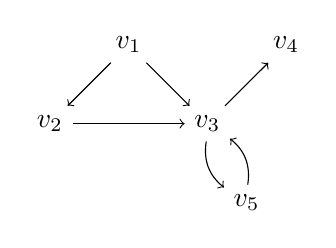
\begin{tikzpicture}
	\node (v1) at (0,0) {$v_1$};
	\node (v2) at (-1,-1) {$v_2$};
	\node (v3) at (1,-1) {$v_3$};
	\node (v4) at (2,0) {$v_4$};
	\node (v5) at (1.5,-2) {$v_5$};

	\path [->] (v1) edge node {} (v2);
	\path [->] (v1) edge node {} (v3);
	\path [->] (v2) edge node {} (v3);
	\path [->] (v3) edge node {} (v4);
	\path [->] (v3) edge[bend right=30] node {} (v5);
	\path [->] (v5) edge[bend right=30] node {} (v3);
\end{tikzpicture}
\end{center}
besitzt die Adjazenzmatrix
\[
A= \begin{bmatrix}
	0 & 1 & 1 & 0 & 0 \\
	0 & 0 & 1 & 0 & 0 \\
	0 & 0 & 0 & 1 & 1 \\
	0 & 0 & 0 & 0 & 0 \\
	0 & 0 & 1 & 0 & 0
\end{bmatrix}
\]
und falls der Graph als ungerichteter Graph aufgefasst wird:
\[
A = \begin{bmatrix}
	0&1&1&0&0\\
	1&0&1&0&0\\
	1&1&0&1&1\\
	0&0&1&0&0\\
	0&0&1&0&0
\end{bmatrix}
\]
\end{example}

\begin{remark}
Bei ungerichteten Graphen ist die Adjazenzmatrix \underline{immer} symmetrisch.\\
Der Speicherbedarf einer Adjazenzmatrix ist $|V|^2$, unabhängig von $|E|$. Für größere Graphen ist dies ineffizient. 
Wir werden beim Behandeln von dünnbesetzten Matrizen ein alternatives Speicherformat kennenlernen. \\
Zum Abschluss bemerken wir, dass sich viele graphentheoretische Konzepte mir Hilfe der Adjazenzmatrix in die Sprach der linearen Algebra übersetzten lässt.
\end{remark}
